%!TEX root = ../template.tex
%%%%%%%%%%%%%%%%%%%%%%%%%%%%%%%%%%%%%%%%%%%%%%%%%%%%%%%%%%%%%%%%%%%
%% chapter2.tex
%% NOVA thesis document file
%%
%% Chapter with Background
%%%%%%%%%%%%%%%%%%%%%%%%%%%%%%%%%%%%%%%%%%%%%%%%%%%%%%%%%%%%%%%%%%%

\typeout{NT FILE chapter2.tex}%

\chapter{Background}
\label{cha:Background}

\prependtographicspath{{Chapters/Figures/Covers/}}

\section{Software Quality}

Quality characteristics are specific properties of software, such as correctness, robustness, readability, and evolvability, which can be measured \cite{MetricsMaintainability1994}. The primary difficulty in improving software quality is not the applicability of a series of good practices but the very foundation that changes with the incorporation of quality from the inception itself in development rather than just depending on testing at the end of development \cite{lientz1980software}.

\subsection{Understanding Dimensions of Software Quality}

Software quality is multi-dimensional and predominantly project-specific, based on individual needs and contexts \cite{MetricsMaintainability1994}. The diverse dimensions include:

\begin{itemize}
    \item \textbf{Correctness:} This refers to the software performing its intended job accurately without errors.
    
    \item \textbf{Robustness:} The software's quality for acting many unintended occurrences without failing. 
    
    \item \textbf{Readability:} Code that is easily readable by new developers, which improves maintainability.

    \item \textbf{Evolvability:} The ease with which software can be changed to accommodate new requirements or environments.
\end{itemize}

Each dimension contributes its unique qualities to the overall software, leading to its long-term success and reliability.

\subsection{Maintenance: The Solution, Not a Problem}

Glass challenges the traditional view that software maintenance is a problem to be minimized therefore not setting it as a priority. Instead, it should be treated as a positive part of the software lifecycle. \cite{MaintenanceGlass1998}. Glass assumes that maintenance is related to enhancements and new functionality added, rather than just error fixing, which is only a small part of maintenance efforts \cite{MaintenanceGlass1998}.

This represents the adaptive and evolutionary nature of software, such that maintenance activities are put in place to ensure continuous improvement and software refinement based on users changing needs and technology advances. Integrating Quality into software development must be incorporated it's life cycle to ensure safety against issues after deployment and ensure maintenance costs are not inflated \cite{osterweil1996strategic} \cite{ManagingMaintenance1983}.
    
\subsection{Lehman’s Laws of Software Evolution}

Lehman’s Laws of Software Evolution provides many insights into the behavior and progression of software over time. Meir M. Lehman and Les Belady formulated these laws based on extensive analysis of industrial engineering projects. We are going to address the two main concerns that most relates to our work:

E-type programs, which are systems that heavily depends on the environment, must continuously adapt to remain functional and satisfactory due to changes in their operational environment. This necessity comes from the cyclical disharmony between the software's present state and its evolving context and not from errors or shortcuts by the engineering team \cite{Lehman1996Laws}. This constant adaptation is driven by the need for feedback and changes in the environment making E-type software similar to biological organisms that must evolve to cope with environmental forces \cite{LehmanLaws1980}.

Over time, software systems inherently become more complex unless continuous efforts are made to control and reduce this complexity. This phenomenon is related to the second law of thermodynamics, where entropy in a closed system continuously increases and every new interaction point within the system increase caused to meet new requirements or fix bugs, the complexity increases \cite{Lehman1996Laws}. If unmanaged, this growing complexity makes maintenance and further development increasingly difficult. Balancing the introduction of new features with complexity management is crucial, though resources for both are limited. Consequently, the rate of growth of a system typically slows as it ages \cite{Lehman1978ProgramsCS}.



\section{Identity Governance and Administration}

Identity Governance and Administration (IGA) is crucial Human Resources activities for managing user data (Name, Position, Contract, etc.), and access. It combines Identity Governance (which focuses on visibility and role management) with Identity Administration (which manages user accounts and provisioning).

The main focus of IGA is to create a secure environment with strict compliance rules to prevent unauthorized access risks managing and controlling user access, enhancing data integrity and confidentiality, and preventing misuse. Other important aspects Tracking the lifecycle of the worker, which handles access rights, Access Governance, that enforces access policies, Access Administration, which manages access requests and reviews, and Role-Based Access Control, that assigns roles based on job responsibilities.


\section{Netwrix Usercube}

Netwrix Usercube is a comprehensive identity and access management solution it enables organizations of all sizes to enhance their security and compliance posture by ensuring the IGA process. The solution make sure access permissions are granted only to those who need them and also managing and automating all types of human resources process, for example, onboarding and offboarding processes, easing the compliance burden.  

The application is better described dividing it in two modules that work together: Identity and Entitlement Management:

\subsection{Identity Management}

A company deals with various identities, including employees and external workers like contractors, who are usually only tracked for billing. All identities requiring work-related entitlements must be represented. Typically, companies use a separate system for each identity type, for example, applications that can be managed by Active Directory (AD) will use the Identity stored on itself but other groups of access have different ways of managing the identy of these users. Usercube consolidates information from multiple source systems to create a central repository that manages all identities throughout their lifecycle. Usercube's repository serves as a mediator between data-providing systems, such as HR systems, and data-receiving systems, like Active Directory.

\begin{figure}[htbp]
  \centering
  \begin{minipage}{0.48\textwidth}
    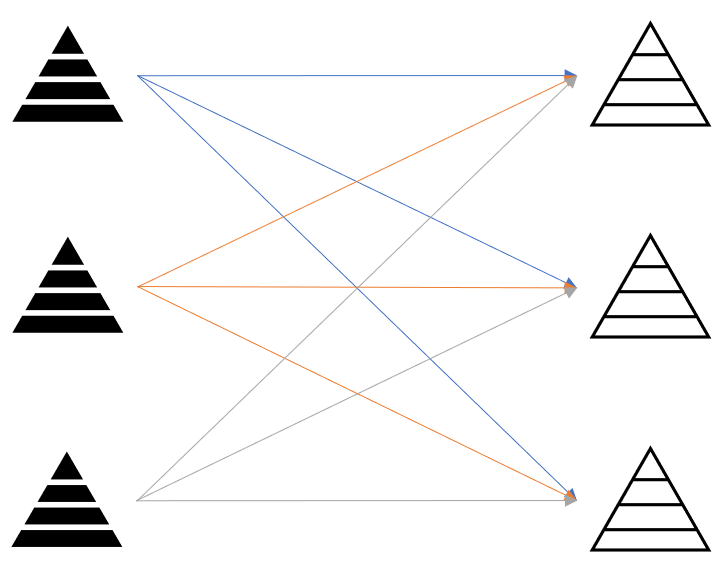
\includegraphics[width=\linewidth]{Identities_complexityQuadratic}
    \caption{Quadratic Complexity}
    \label{fig:Identities_complexityQuadratic}
  \end{minipage}\hfill
  \begin{minipage}{0.48\textwidth}
    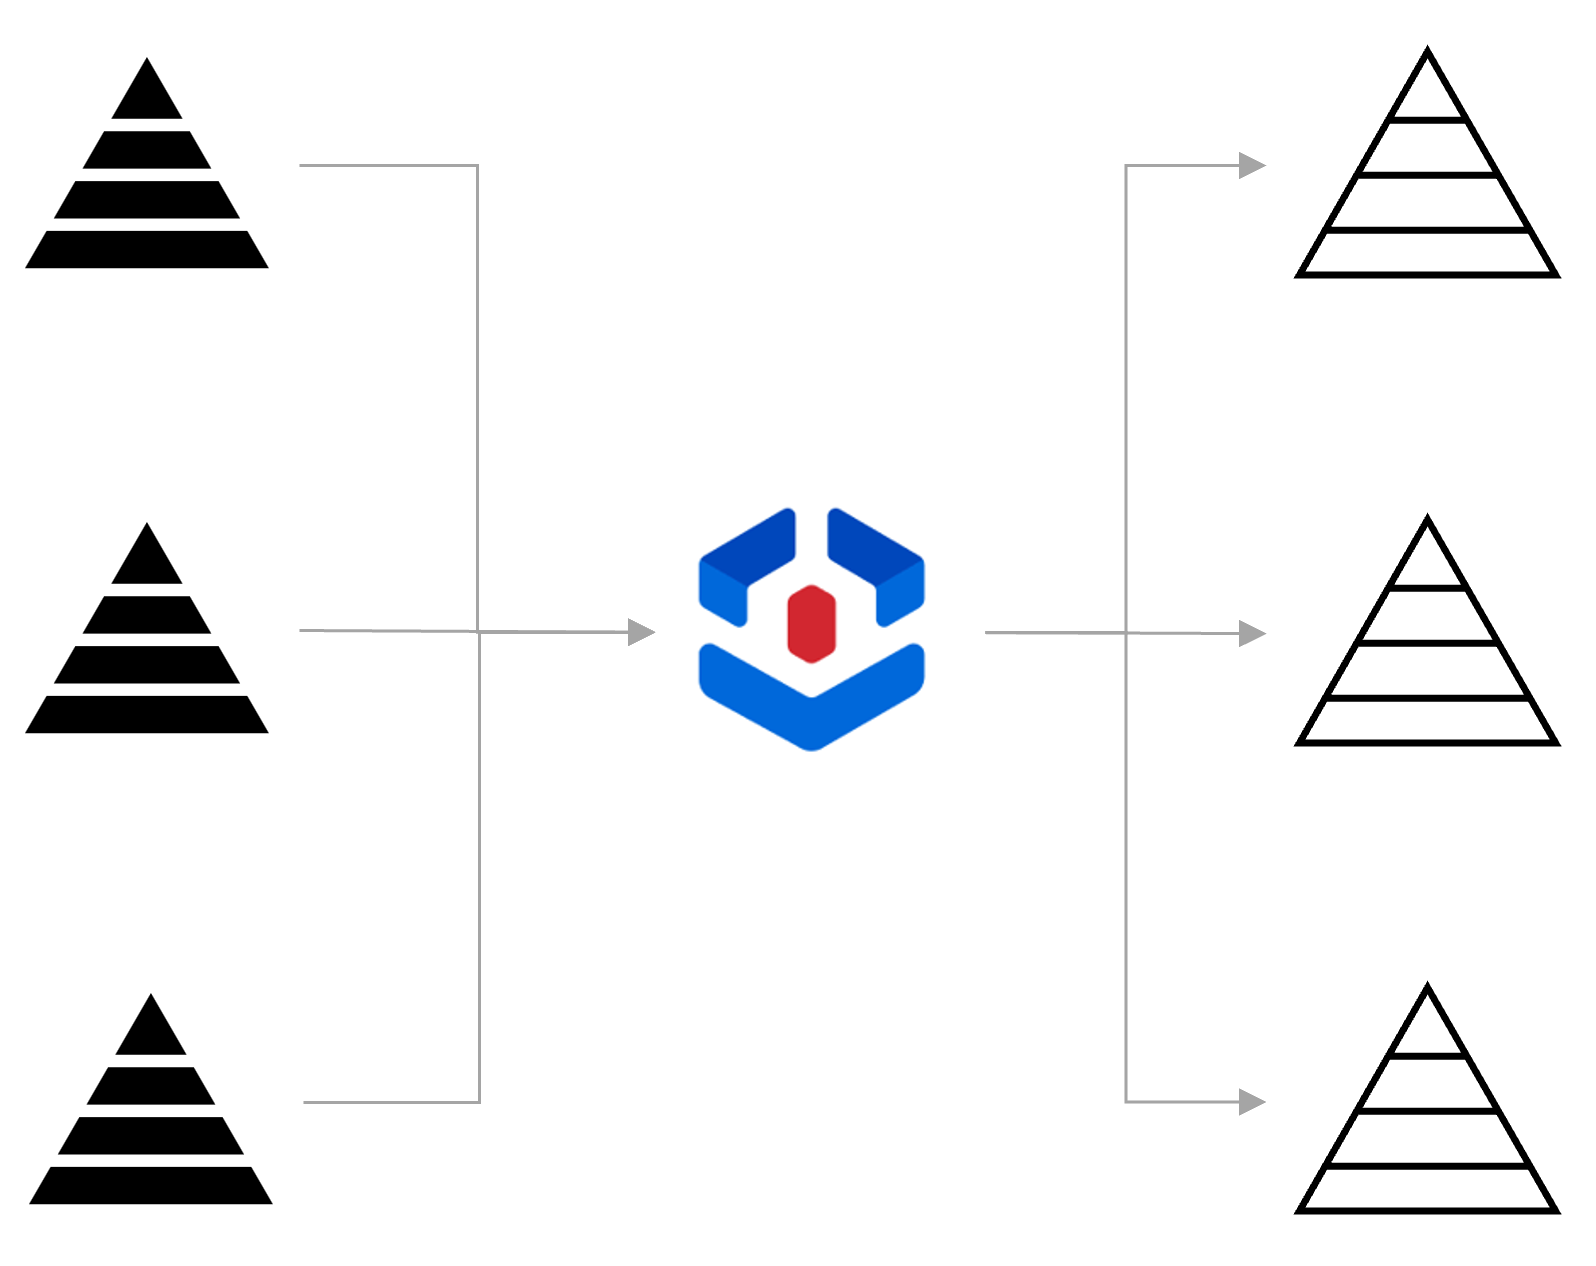
\includegraphics[width=\linewidth]{Identities_complexityLinear}
    \caption{Linear Complexity}
    \label{fig:Identities_complexityLinear}
  \end{minipage}
\end{figure}

As we can see in the representation, with a central repository, adding a new system needs only one additional set of rules, making the complexity linear but without an intermediary, adding a new system to n systems requires n sets of rules, resulting in quadratic complexity \cite{UsercubeDocument}.

\subsection{Entitlement Management}

Entitlement Management involves assigning entitlements to identities, which are permissions allowing access to specific data, location or application. In systems like Active Directory, entitlements often manifest as group memberships. Usercube is a tool designed to manage these entitlements by creating a comprehensive catalog and ensuring correct assignments based on a role model that includes governance data and risk definitions \cite{UsercubeDocument}.

In Usercube, entitlements are represented as roles within a role catalog that lists all entitlements from managed systems \cite{UsercubeDocument}. These roles are linked to specific provisioning rules that write the actual entitlements to the systems, automating the assignment process. For example, to assign an Active Directory entitlement, a rule might add a user to a particular group when a role is assigned via the application interface. Assignment rules in Usercube automatically assign roles to users based on criteria like job title and location, ensuring compliance and helping as well flagging incongruent assignments as non-conforming.

Usercube manages different resources through categorized rules, distinguishing between resource types such as standard and administration accounts. This categorization allows for differentiated management, such as setting distinct email addresses and approval workflows for privileged accounts, enhancing security.

\begin{figure}[htbp]
  \centering
  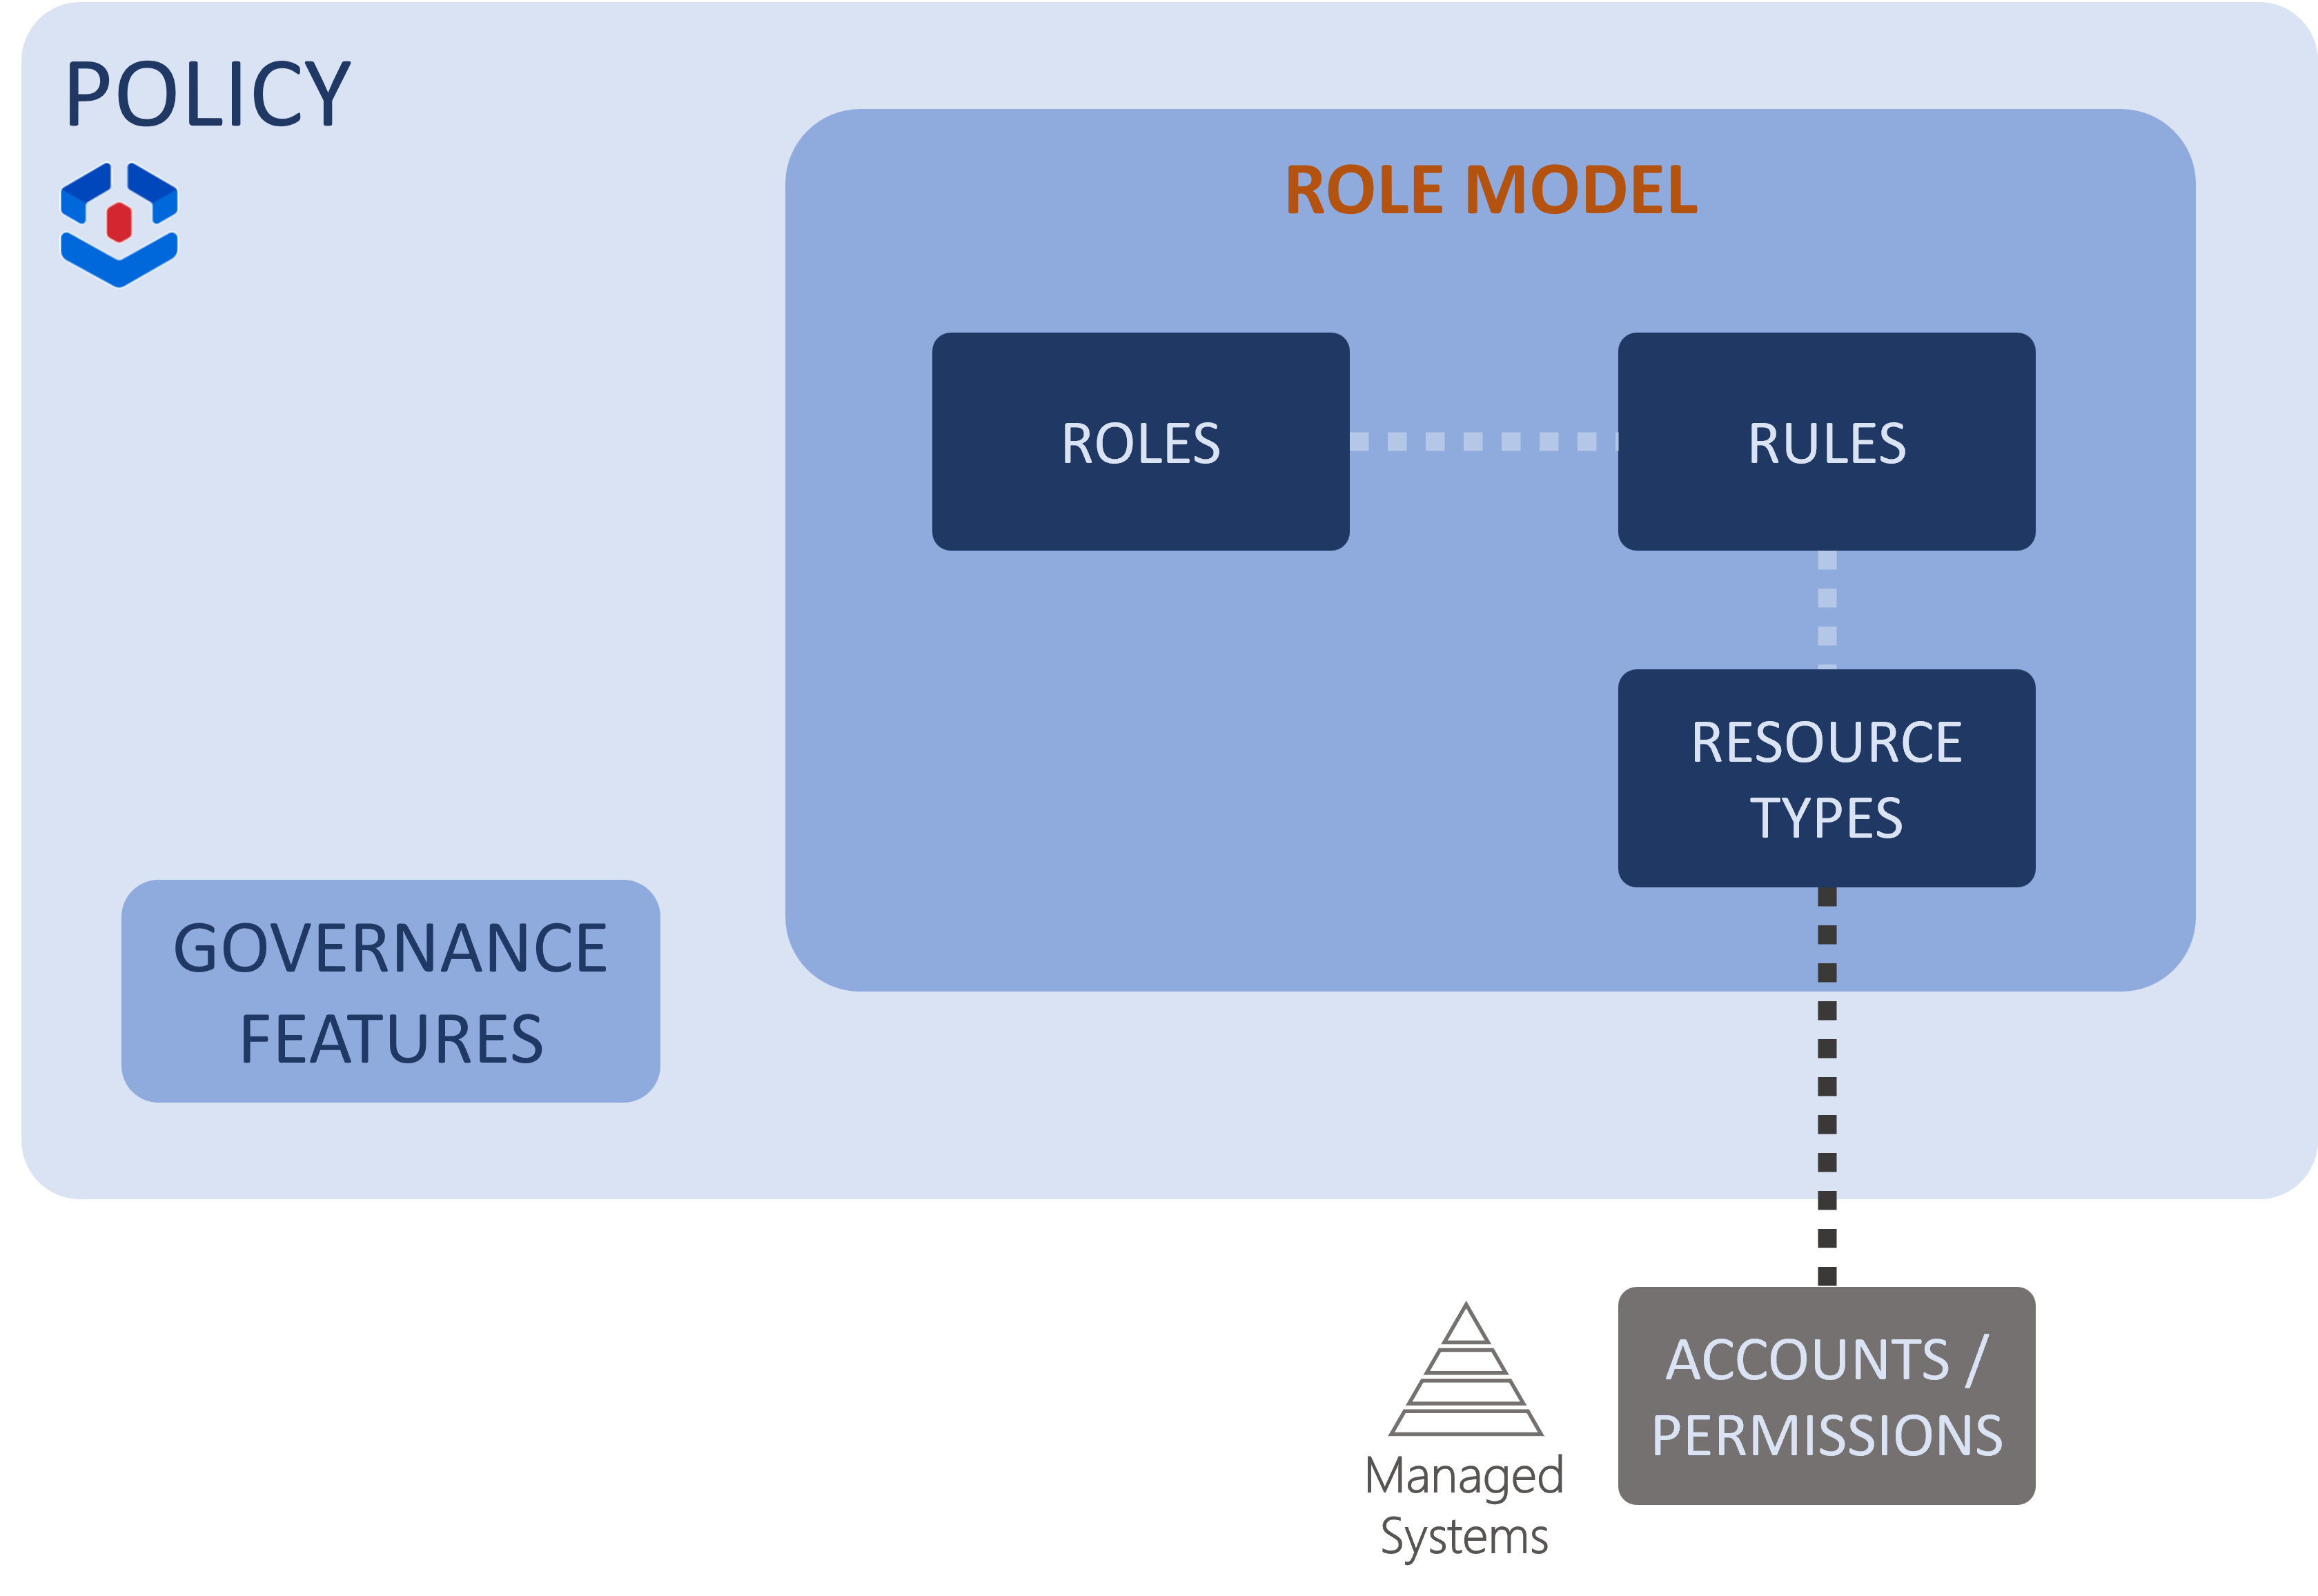
\includegraphics[width=5in]{Entitlements_RoleModel}
  \caption{Entitlements Role Model}
  \label{fig:Entitlements_RoleModel}
\end{figure}

\subsection{Architecture}

Usercube works via a server which operates computation, stores all application data in the database, and serves a web User Interface; at least one agent which operates data flows to/from the managed systems. The managed systems credentials are used only by the agent and are never revealed to the server. The agent can call the server, but the server cannot call the agent. The data flow initiatives are always from the agent. In our case the installation is on-premises so that the server is installed on an isolated network within the group infrastructure that is managed by the another department.

\begin{figure}[htbp]
  \centering
  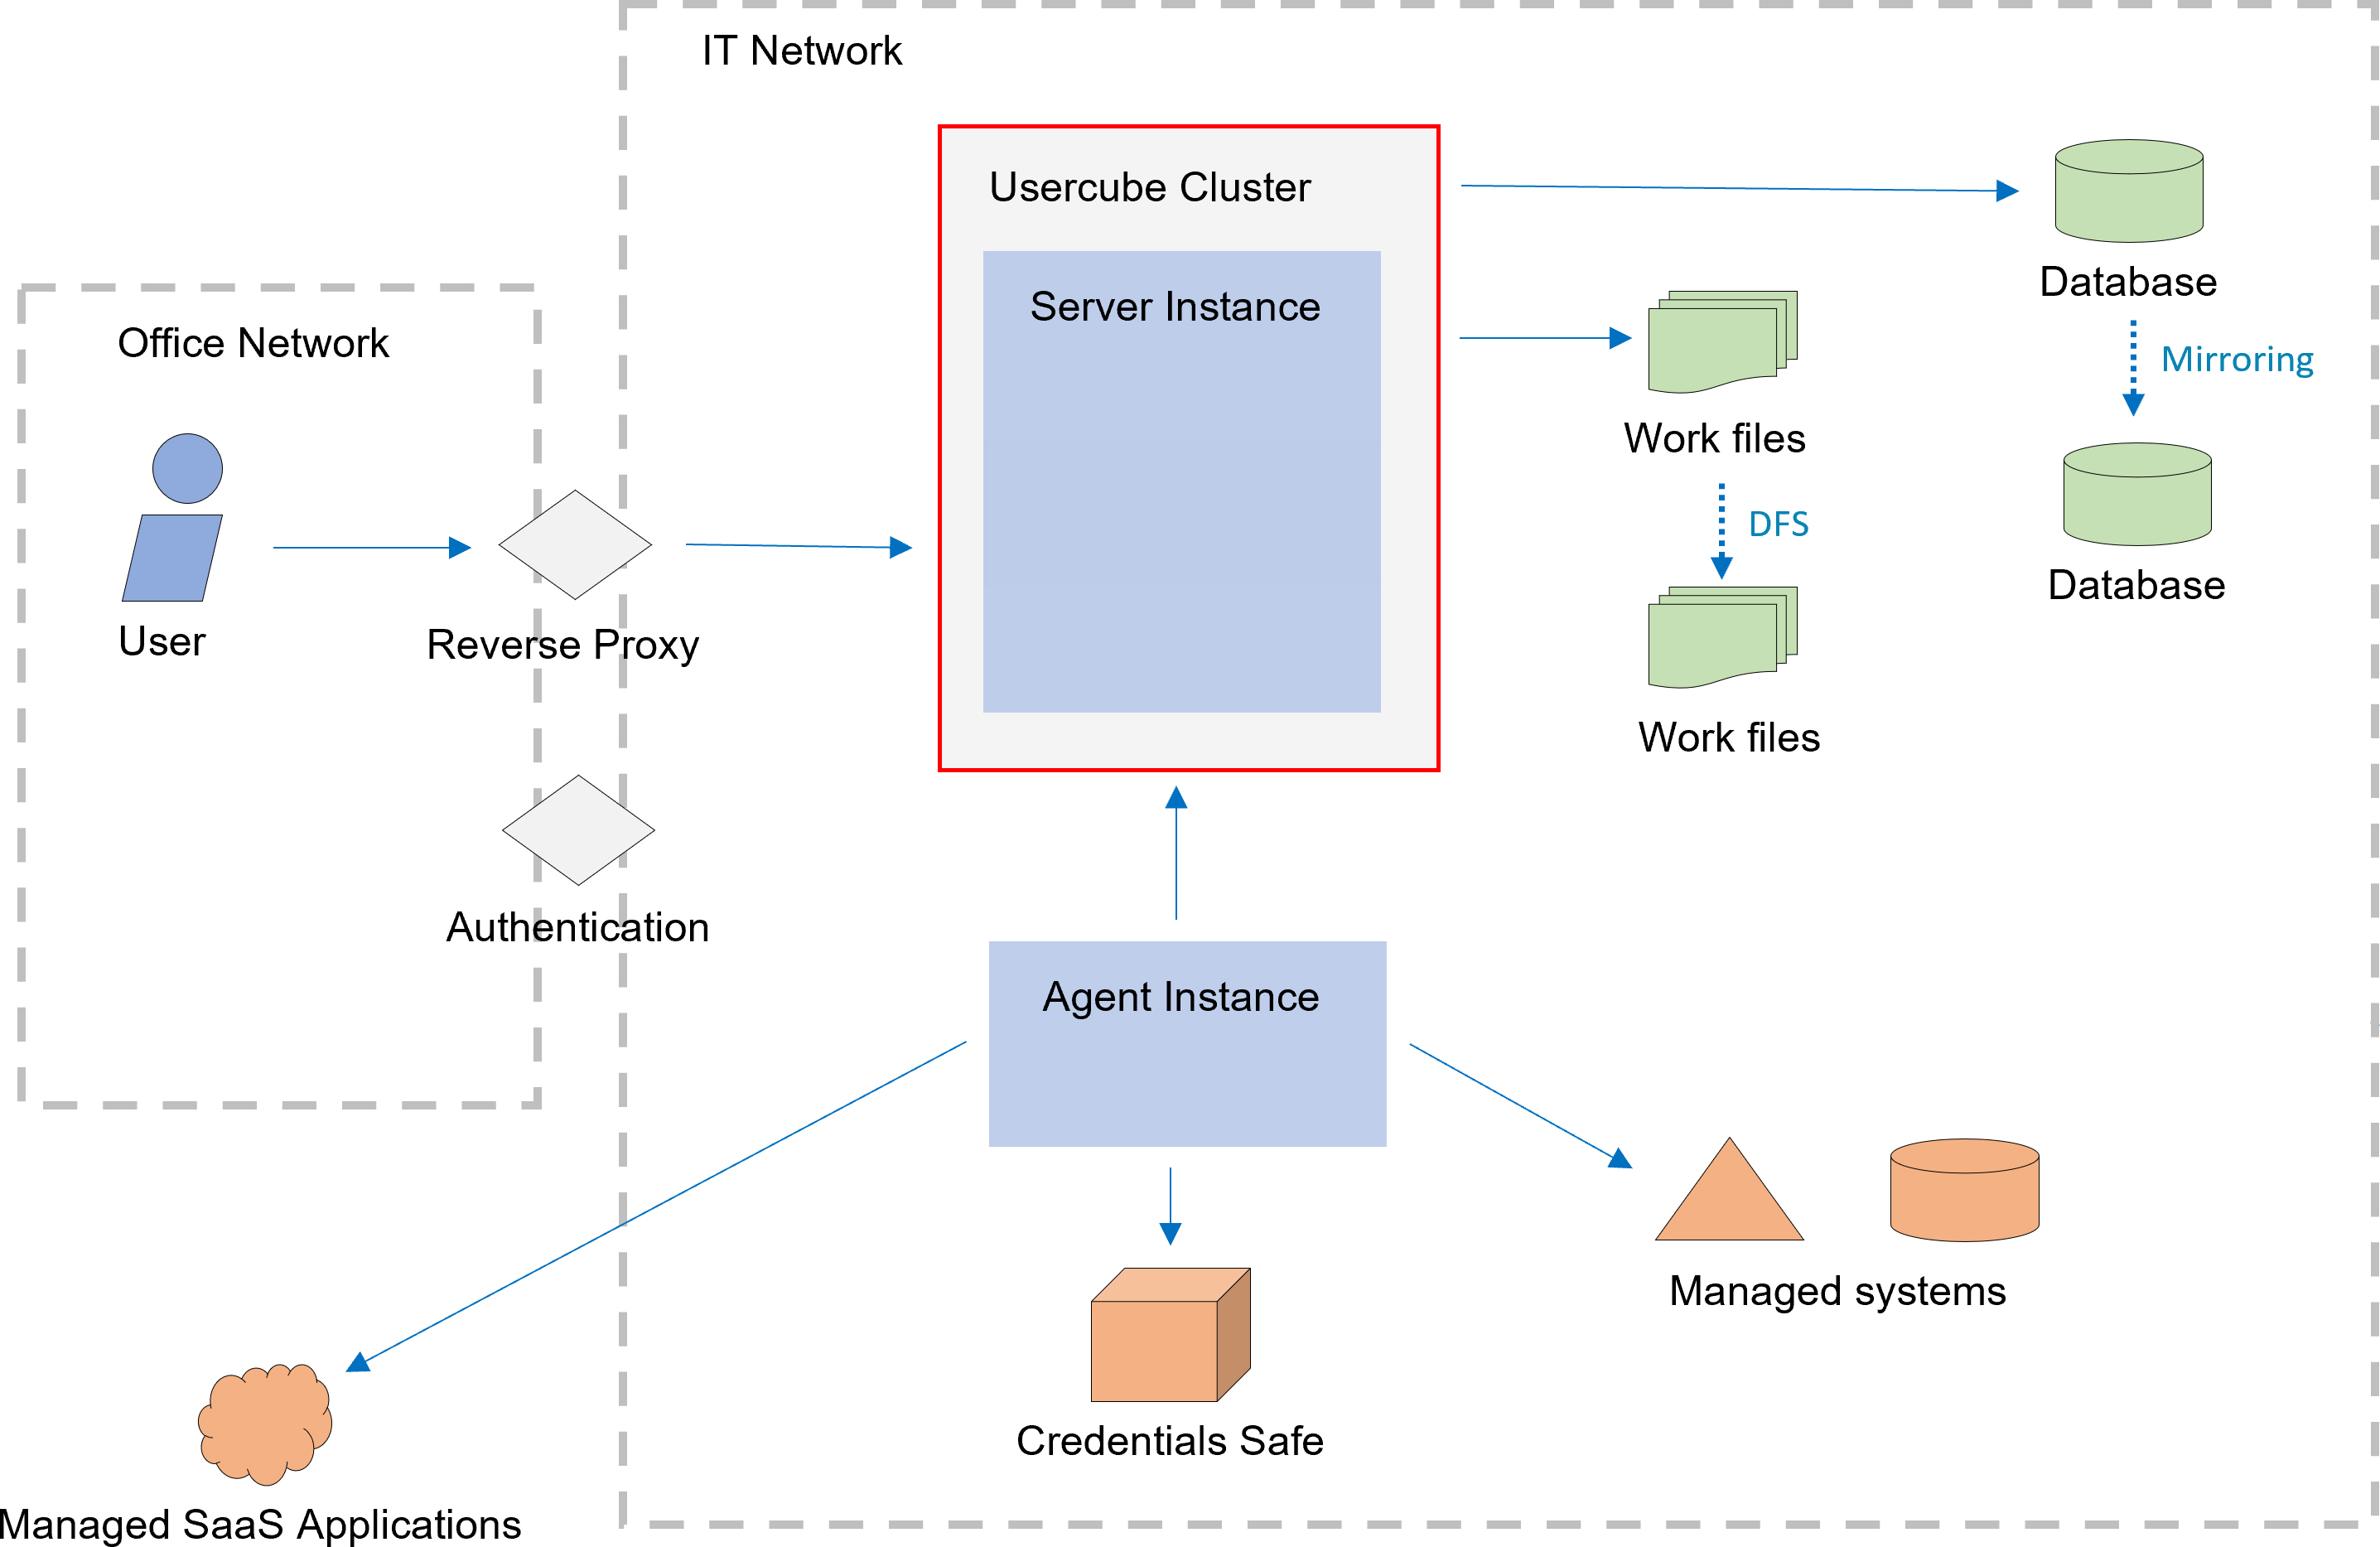
\includegraphics[width=5in]{Architecture_onPrem}
  \caption{Architecture on premises, adapted \cite{UsercubeDocument}.}
  \label{fig:Architecture_onPrem}
\end{figure}

Users initiate a interation via the UI that pass through a reverse proxy for secure traffic direction, followed by an authentication. After successful authentication, requests are handled by a Usercube cluster, comprising server instances that act as the central management hub. This cluster interfaces with an agent instance responsible for managing the connections to various systems. The agent also connects to managed systems, such as databases.

\subsection{Configuration}

A Usercube configuration consists of a set of XML files structured according to the Usercube schema and it is stored in the Usercube database and utilized at runtime. These files serves to define and manage various elements of the application, such as entities, properties, profiles, access control rules, etc. 

Although the XML configuration schema shares some similarities with the database schema they have distinct ways to represent the data. This method of configuration offers flexibility and control for developers who need to manage the implementation of complex policies or integrate Usercube with other systems.

To illustrate the configuration elements some good examples would be a new Entity Type definition. This involves defining the structure of the data entities managed by Usercube, each entity type is described using XML elements that specify its properties and their characteristics. The entity type have individual attributes called properties. Every entity type generates a new view on the database where the information will be available after the deployment.


\begin{lstlisting}[language=XML, caption=Definition of the User Entity Type example]
<EntityType Identifier="User">
    <Property Identifier="Name" TargetColumnIndex="15" Type="String" />
    <Property Identifier="HasCard" TargetColumnIndex="61" Type="Bool" />
</EntityType>
\end{lstlisting}

Another important aspect is for example the assertion elements designed to check if the value of a given property meets a specified condition. It involves defining expressions to validate property values during certain workflow activities, with the capability to handle both single and multi-valued objects. The validation is triggered by the PointCut elements that define in which state of the assertion should be done.

\begin{lstlisting}[language=XML, caption=AssertValueAspect element example to check a date]
    <AssertValueAspect Identifier="Directory_User_NewInternal_CheckDates" 
        Binding="Workflow_Directory_User:Directory_User.Records.ContractEndDate" 
        ExpressionBinding="Workflow_Directory_User:Directory_User.Records"
        Expression="C#:record: return ( 
            ((Nullable&lt;DateTime&gt;) record.ContractStartDate).HasValue &&
            ((Nullable&lt;DateTime&gt;) record.ContractEndDate).HasValue) ?
            record.ContractStartDate &lt; record.ContractEndDate : true;"
        Message_L1="Contract's end date must be after contract's start date.">
        <PointCut Activity="Directory_User_NewInternal:Request"
            ActivityState="ActionWithRefine-Executed" Mode="Before" />
        <PointCut Activity="Directory_User_NewInternal:Review"
            ActivityState="ReviewWithFeedback-Approved" Mode="Before" />
    </AssertValueAspect>
\end{lstlisting}

When the XML files are ready to be tested, a command start the process of compilation where the configuration are going to be analysed and verified against the XSD file containg all the restrictions of the XML files and error messages that are shown in the console if any mistake was made.

\begin{lstlisting}[language=sh, caption=Shell command to execute the configuration delpoy]
./Usercube-Deploy-Configuration.exe  --configuration-directory "C:/Usercube/ExportedConf"
\end{lstlisting}

After the verification of the files is done, the application is going to import all elements and properties into the date base, triggering storage procedures that are going to break down these elements and it is going to add the information to the respective table.

\begin{figure}[htbp]
  \centering
  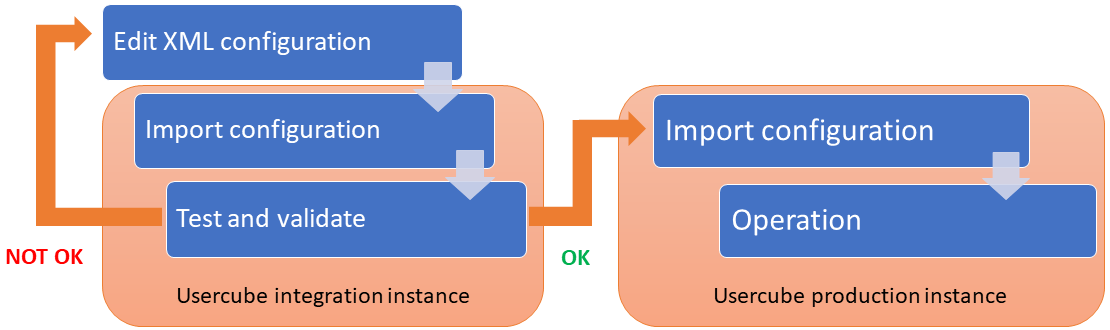
\includegraphics[width=5in]{configurationCycle}
  \caption{Usercube's configuration Cycle}
  \label{fig:configurationCycle}
\end{figure}

\subsection{XML Configuration and Object-Oriented Programming (OOP)}

The structural and functional paradigms of XML schema configurations in Usercube share similarities to the principles of Object-Oriented Programming (OOP). In the XML configuration, elements encapsulate specific configuration details, similar to how classes in OOP encapsulate data and methods. This encapsulation allows each XML tag to define distinct aspects of the configuration, mirroring the way class definitions manage properties and behaviors.

The modular approach present in the XML configurations facilitates the definition and reuse of individual components. This modular construction relates to the structure of OOP, where classes and objects can be defined once and reused across different parts of a program, promoting maintainability and scalability.

The hierarchical structure is conceptually similar to class inheritance and object composition in OOP as well. In XML, parent elements encompass child elements, establishing a nested relationship that reflects the hierarchical arrangement of base and derived classes or the composition of objects within larger objects.

In XML, configurations are designed to define components like entity types or profiles that are applicable across various application segments, comparable to how classes and methods are designed to be reusable in OOP. This reusability extends functionality without necessitating redundancy, thereby streamlining development processes.

Lastly, abstraction in XML configurations simplifies complex settings into more manageable components. This abstraction mirrors OOP’s methodology of hiding implementation details behind interfaces and class definitions, making complex systems easier to manage and adapt.
